\documentclass[12pt]{article}
\usepackage[utf8]{inputenc}
\usepackage[
    left=2.5cm,
    right=2.5cm,
    top=4cm,
    bottom=4cm
]{geometry}
\usepackage{courier}
\usepackage{listings}
\usepackage{tocloft}
\usepackage{xcolor}
\usepackage{amsmath}
\usepackage{mathtools}
\usepackage{amsfonts}
\usepackage{fancyhdr}

\allowdisplaybreaks

\definecolor{pOrange}{RGB}{248,174,33}
\lstset{
	basicstyle=\footnotesize\ttfamily,
	breaklines=true, 
	numbers=left, 
	language=Python, 
	tabsize=2, 
	moredelim=**[is][\color{green}]{\$}{\$},
	moredelim=**[is][\color{pOrange}]{!}{!},
	moredelim=**[is][\color{red}]{~}{~}
}
\definecolor{greenJS}{rgb}{0,0.6,0}
\definecolor{grayJS}{rgb}{0.5,0.5,0.5}
\definecolor{mauveJS}{rgb}{0.58,0,0.82}
 
%Customize a bit the look

%END of listing package%
 
\definecolor{darkgrayJS}{rgb}{.4,.4,.4}
\definecolor{purpleJS}{rgb}{0.65, 0.12, 0.82}
 
%define Javascript language
\lstdefinelanguage{JavaScript}{
	keywords={typeof, new, true, false, catch, function, return, null, catch, switch, var, if, in, while, do, else, case, break},
	keywordstyle=\color{blue}\bfseries,
	ndkeywords={class, export, boolean, throw, implements, import, this},
	ndkeywordstyle=\color{darkgrayJS}\bfseries,
	identifierstyle=\color{black},
	sensitive=false,
	comment=[l]{//},
	morecomment=[s]{/*}{*/},
	commentstyle=\color{purpleJS}\ttfamily,
	stringstyle=\color{red}\ttfamily,
	morestring=[b]',
	morestring=[b]"
}
 
\renewcommand{\cftsecleader}{\cftdotfill{\cftdotsep}}

% Github style syntax highlighting
\newcommand{\highlight}{\colorbox{gray!10}}

% Does anyone like bullet points?
\def\labelitemi{--}

\setlength{\headheight}{15.0pt}
\pagestyle{fancy}
\lhead{Jing C. Lin}
\chead{Problem Set 1}
\rhead{Fall 2015}

\begin{document}
\setlength{\parindent}{0pt}\par{Collaborators: Alisa Ono. Written Sources: Textbook}
\subsection*{Problem 1}
\par{Prove that $\log_4 6$ is irrational.}
\newline
\par{Proof by contradiction.}
\par{Assume that $\log_4 6$ is rational. Therefore, by the definition of a rational number, it can be expressed as a fraction $\frac{m}{n}$ where $m, n \in Z$.}
\begin{align*}
\log_4 6 &= \frac{m}{n} \\
n * \log_4 6 &= m \\
4^{n * \log_4 6} &= 4^m \\
(4^{\log_4 6})^n &= 4^m \\
6^n &= 4^m \\
3^{2n} &= 2^{2m} \\
3^{n'} &= 2^{m'}
\end{align*}
\par{Since the LHS has a factor of 3 and the RHS has a factor of 2, it's impossible for the two to ever be equal. Therefore, we've arrived at a contradiction and our initial assumption that $\log_4 6$ is rational is False. Therefore it's irrational.}

\subsection*{Problem 2}
\par{Use the Well Ordering Principle to prove that $n \leq 3^{\frac{n}{3}}$ for every nonnegative integer, $n$.}
\newline
\par{Let's first define the predicate $P(n) = n \leq 3^{\frac{n}{3}}$.}
\par{Let's now define $C$.}
\begin{align*}
C ::= \{n \in N^+ | \text{NOT}(P(n))\}
\end{align*}
\par{Proof by contradiction. Assume that C is a nonempty set. Therefore, by the WOP, there exists a minimum element $n'$ in $C$. Let's check a few cases now.}
\begin{align*}
P(0) &= 0 \leq 3^{\frac{0}{3}} \\
&= 0 \leq 1 \\
&= \text{True} \\
P(1) &= 1 \leq 3^{\frac{1}{3}} \\
&= 1 \leq 1.42... \\
&= \text{True} \\
P(2) &= 2 \leq 3^{\frac{2}{3}} \\
&= 2 \leq 2.08... \\
&= \text{True} \\
P(3) &= 3 \leq 3^{\frac{3}{3}} \\
&= 1 \leq 1 \\
&= \text{True}
\end{align*}
\par{We'e shown that $n' \geq 3$ which means that $P(n' - 3)$ is True since $n'$ is the minimum element in $C$ and any nonnegative element lower than $n'$ is not in $C$. Writing that out, we know that}
\begin{align*}
P(n' - 3) &= \text{True} \\
n' - 3 &\leq 3^{\frac{n' - 3}{3}} \\
n' &\leq 3^{\frac{n' - 3}{3}} + 3 \\
n' &\leq 3^{\frac{n'}{3}} \\
= P(n')
\end{align*}
\par{Since we previously assumed $P(n')$ is not True and it's actually True, our assumption that $C$ is nonempty is False and $P(n)$ does hold for every nonnegative integer.}

\subsection*{Problem 3}
\par{\textbf{a.} Verify by truth table that $(P\;\;\text{IMPLIES}\;\;Q)\;\;\text{OR}\;\;(Q\;\;\text{IMPLIES}\;\;P)$ is valid.}
\begin{center}
	\begin{tabular}{c|c|c|c|c}
	$P$ & $Q$ & $P \rightarrow Q$ & $Q \rightarrow P$ &$P \rightarrow Q\;\;\text{OR}\;\;Q \rightarrow P$ \\
	\hline
	T & T & T & T & T \\
	T & F & F & T & T \\
	F & T & T & F & T \\
	F & F & T & T & T \\
	\end{tabular}
\end{center}
\par{\textbf{b.} Let $P$ and $Q$ be propositional formulas. Describe a single formula, $R$ using only AND, OR and NOT and copies of $P$ and $Q$ such that $R$ is valid iff $P$ and $Q$ are equivalent.}
\newline
\par{$P$ and $Q$ are equivalent only when their truth values are the same for all cases. Therefore, $R = P \\arrow Q$.}
\begin{align*}
P \rightarrow Q &= (\text{NOT}(P)\;\;\text{OR}\;\;Q) \\
Q \rightarrow P &= (\text{NOT}(Q)\;\;\text{OR}\;\;P) \\
R &= (P \rightarrow Q)\;\;\text{AND}\;\;(Q \rightarrow P) \\
R &= (\text{NOT}(P)\;\;\text{OR}\;\;Q)\;\;\text{AND}(\text{NOT}(Q)\;\;\text{OR}\;\;P)
\end{align*}
\par{\textbf{c.} A propositional formula is \textit{satisfiable} iff there is an assignment of truth values to its variables, an \textit{environment}, which makes it true. Explain why $P$ is valid iff NOT($P$) is \textit{not} satisfiable.}
\newline
\par{There are two cases to consider, when P is True and when P is False. In the first case, P is True.}
\begin{align*}
T \leftrightarrow F &= \text{False}
\end{align*}
\par{In the second case, P is False.}
\begin{align*}
F \leftrightarrow T &= \text{False}
\end{align*}
\par{\textbf{d.} A set of propositional formulas $P_1, \cdots P_k$ is \textit{consistent} if there is an environment in which they are all True. Write a formula S so that the set $P_1, ... P_k$ is not consistent iff S is valid.}
\begin{align*}
S = \text{NOT}(P_1\;\;\text{AND}\;\;P_2\cdots\text{AND}\;\;P_k)
\end{align*}
\par{Here $S$ can only be valid iff set of propositions is not consistent.}

\subsection*{Problem 4}
\par{There are adder circuits that are \textit{much} faster, and only slightly larger, than the ripple-carry circuits of Problem 3.5 of the course text. They work by computing the values in later columns for both a carry of 0 and a carry of 1, in \textit{parallel}. Then, when the carry from the earlier columns finally arrives, the precomputed answer can be quickly selected. We'll illustrate this idea by working out the equations for an $(n + 1)$-bit parallel half-adder.}
\newline
\par{Parallel half-adders are built out of parallel \textit{add1} modules. An (n + 1)-bit \textit{add1} module takes as input the $(n + 1)$-bit binary representation, $a_n\cdots a_1a_0$ of an integer $s$, and produces as output the binary representation $c p_n\cdots p_1 p_0$, of $s + 1$.}
\newline
\par{\textbf{a.} A 1-bit \textit{add1} module just has input $a_0$. Write propositional formulas for its output $c$ and $p_0$.}
\begin{align*}
p_0 &= a_0\;\;XOR\;\;1 \\
c &= a_0
\end{align*}
\par{\textbf{b.} Explain how to build an $(n + 1)$-bit parallel half-adder from an $(n + 1)$-bit \textit{add1} module by writing a propositional formula for the half-adder output $o_i$ using only the variables $a_i, p_i$ and $b$.}
\newline
\par{The half-adder output $o_i$ is dictated by the value of $b$. If $b = 1$, then $o_i = p_i$. If $b = 0$, then $o_i = a_i$. The statements are correspondingly translated to:}
\begin{align*}
o_i &= ((\text{NOT}(b)\;\;\text{OR}\;\;p_i)\;\;\text{AND}\;\;b))\;\;\text{OR}\;\;((b\;\;\text{OR}\;\;a_i)\;\;\text{AND}\;\;\text{NOT}(b)) \\
o_i &= ((b)\;\;\text{AND}\;\;p_i)\;\;\text{OR}\;\;((\text{NOT}(b)\;\;\text{AND}\;\;a_i)
\end{align*}
\par{\textbf{c.} We can build a double-size \textit{add1} module with $2(n + 1)$ inputs using two single-size \textit{add1} modules with $n + 1$ inputs. Suppose the inputs of the double-size module are $a_{2n + 1}\cdots,a_1a_0$ and the outputs are $c,p_{2n + 1}\cdots,p_1,p_0$. The setup is illustrated in the Figure below.}
\newline
\par{Namely, the first single size \textit{add1} module handles the first $n + 1$ inputs. The inputs to this module are the low-order $n + 1$ input bits $a_n\cdots a_1,a_0$ and its outputs will serve as the first $n + 1$ outputs $p_n\cdots,p_1,p_0$ of the double-size module. Let $c_{(1)}$ be the remaining carry output from this module.}
\newline
\par{The inputs to the second single size \textit{add1}} module are the higher order $n + 1$ input bits $a_{2n + 1}\cdots,a_{n + 2},a_{n + 1}$. Call its first $n + 1$ outputs $r_n,\cdots,r_1,r_0$ and let $c_{(2)}$ be its carry.
\begin{figure}[h]
	\centering
	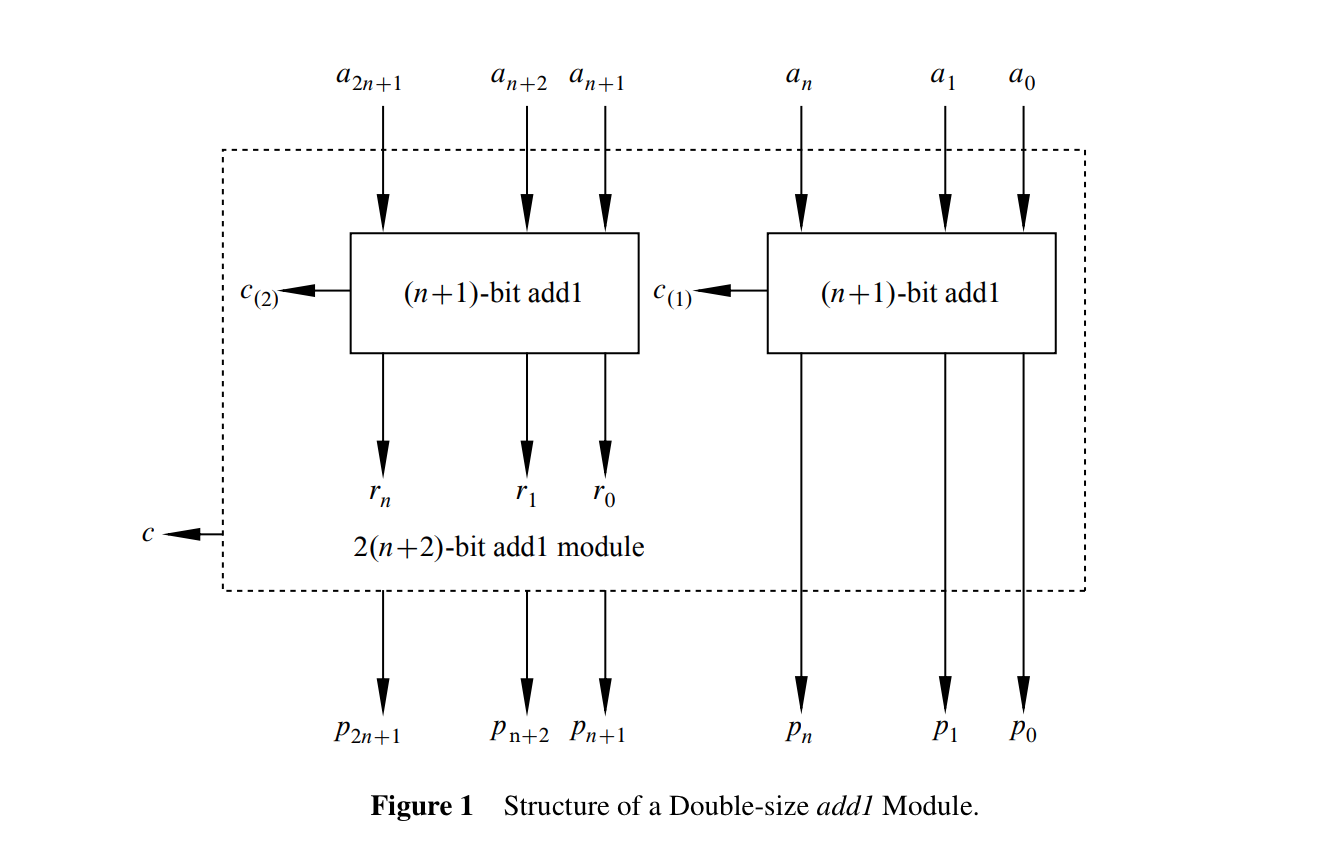
\includegraphics[width=0.7\linewidth]{1_double_sized_adder.png}
\end{figure}
\par{Write a formula for the carry, $c$ in terms of $c_{(1)}, c_{(2)}$.}
\newline
\par{There are a few cases to consider. If $c_{(1)}$ is zero, then it doesn't matter what the value of $c_{(2)}$ was because $c_{(2)}$ should be zero. If $c_{(1)}$ is one, then the carry $c$ is only equal to one when $c_{(2)}$ is also one. Therefore the formula is}
\begin{align*}
c &= c_{(1)}\;\;\text{AND}\;\;c_{(2)}
\end{align*}
\par{\textbf{d.} Complete the specification of the double-size module by writing propositional formulas for the remaining outputs, $p_i$ for $n + 1 \leq i \leq 2n + 1$. The formula for $p_i$ should only involve the variables $a_i, r_{i - (n + 1)}$ and $c_{(1)}$.}
\newline
\par{Intuitively, if $c_{(1)}$ is zero, then $p_{n + i}$ should be equal to the input $a_{n + i}$. Else, it should be equal to the current output $r_{i - 1}$. Translating that into propositional logic, we have}
\begin{align*}
P_{n + i} &= ((\text{NOT}(c_{(1)})\;\;\text{OR}\;\;r_{i - (n + 1)})\;\;\text{AND}\;\;c_{(1)})\;\;\text{OR}\;\;((c_{(1)}\;\;\text{OR}\;\;a_{n + i})\;\;\text{AND}\;\;\text{NOT}(c_{(1)})) \\
&= (r_{i - (n + 1)})\;\;\text{AND}\;\;c_{(1)})\;\;\text{OR}\;\;(a_{n + i}\;\;\text{AND}\;\;\text{NOT}(c_{(1)}))
\end{align*}
\par{\textbf{e.} Parallel half-adders are exponentially faster than ripple-carry half-adders. Confirm this by determining the largest number of propositional operations required to compute any one output bit of an n-bit add module.}
\newline
\par{Since there are 4 operations to determine any $P_{n + i}$ and there are $\log{n}$ levels, there are at most $4\log{n}$ propositional operations which is significantly faster than conventional \textit{add1} modules.}
\end{document}


